\section{Methodology}
\label{sec:methodology}

To achieve the specific objectives, three modules: mechanical, electrical, and control will have to be developed in a synergistic manner. 

\subsection{Mechanical Module}

\subsubsection{Castor Wheels}

Several considerations need to be taken into account when selecting the type of castors to use, the most important being the load capacity of the wheel.
This will be determined by the diameter of the wheel.
The castor should also be easy to modify to achieve motion from a motor.

\subsubsection{Mechanical chassis and platform}

The chassis will form the underside of the mobile platform and will be used to attach the caster wheels and their drive systems.
It will also hold platform onto which the electrical and electronic components, including the motors and control unit will be supported.
The platform will cover up the electronics and allow for an application to be added to the system.
The two modules will be made from the same material, preferably metal. 
Some of the design considerations for this material are:

\begin{itemize}

    \item It should be lightweight and able to handle heavy loads, i.e., it should have excellent tensile strength.
    
    \item It should have high machinability which would make fabrication easy.
    
    \item It should have corrosion resistance.
    
    \item It should be readily available.
    
\end{itemize}

These design considerations narrow down the list of appropriate materials to aluminium, steel, and stainless steel.
The metal that satisfies these considerations will be selected for the design work.

\subsubsection{Power Transmission Unit}

To transmit power from the motor to the wheels, a power transmission unit will be required.
The mechanical power transmission elements under consideration are shafts and couplings, gears and gear trains, brakes and clutches, and chains.
Some of the things to consider when assembling a power transmission unit are:

\begin{itemize}
    
    \item Torque transmitted
    
    \item Parallel or non-parallel shafts
    
    \item Shaft size
    
    \item Speed of rotation
    
\end{itemize}

The mechanical shaft is the most important part of the power transmission unit.
Sub-components such as couplings, gears, and chains are mounted onto a shaft to transmit power or rotation from a motor.
The connection should ensure the connection transmits the load, power and rotation without slipping and within the accuracy requirement of the design.
Load, power, and rotation speeds will be determined from the motor characteristics.

\subsection{Electrical and Electronics Module}

\subsubsection{Motors}
The motor is the main actuation unit in the system.
Each wheel will have its own independent actuation unit made up of motors and power transmission components.
In particular, \ac{DC} motors will be used, and several parameters of the motor will be considered before settling on a final design.
Some of these parameters are horsepower, rotation speed, and maximum torque.
These characteristics will depend on the mechanical structure of the mobile platform.
The size, weight, and maximum load characteristics will ultimately determine the motor speed, torque, and power requirements. 
The choice of motor will also depend on : 

\begin{itemize}

    \item Maximal speed.
    The duration of how long it takes to have the sustained maximum speed needs to be calculated.
    If we are using a gearbox, the available gear ratios will help us calculate the maximal speed of the motor
    \item Maximal torque.
    The maximum torque enables the vehicle to start in a given slope.
    It is possible to calculate the highest torque required by the electric motor considering the differential and gearbox, if using a gearbox.
    Maximal weight is also to be taken into consideration.
        
    \item Maximal power.
    The maximum power is found simply at maximum speed, this is the case where the vehicle as a large frontal area or goes at very high speed.
    This translates to having a motor powerful enough to go through all the different conditions the vehicle can be submitted to.
    The maximum power enables the vehicle to reach and maintain a constant speed under stringent slope and speed conditions.
    To calculate the maximum power, you need to have a simulator that takes in account the drag and friction coefficients of the vehicle in addition to the forces needed for the climb.
    
    \item Battery Capacity.
    The battery capacity is typically calculated using a simulator to go through a reference cycle typical of the usage of the vehicle.
    The simulator can output the consumption of the vehicle in Wh/m.
    
    \item Battery Voltage.
    The battery voltage is dependent on the size of the vehicle.
    As the battery voltage increases, the current output is lowered.
    So in the cases where the vehicle continuous power is high like in bigger vehicles, you want to keep the size of the conductors at a manageable level by increasing the battery voltage.

    \item Gearbox or direct-drive.
    The high torque/low speed of the motor allows it to directly interface with standard axle differentials without the need for an intermediate gearbox.
    While improving system reliability and reducing overall maintenance costs.
    
    \item Cost
    
\end{itemize}

\subsection{Control Module}

\subsubsection{Processing Unit}

Responsible for executing the application logic, sending instructions to the motor driver, and reading inputs from the proximity sensors in the system.
The choice of a micro controller or microprocessor will be determined by the following factors.

\begin{itemize}
    \item Analog Pins:
    This is the interface between the motor driver and the control module.
    The analog pins should be able to send the different modes to the motors attached to the motor driver.
    The availability of approximately 16 will guide the choice of micro controller needed
    
    \item \ac{DAC} Resolution
    Since we need a fine grain control of speed on the motors we will therefore need a micro controller or microprocessor with a higher \ac{DAC} resolution.
    
    \item Wireless capability: 
    Since we need the mobile platform to be remotely actuated we need a micro controller that can be able to connect to a wireless standard preferably WiFi or Bluetooth low energy.
    The availability of this two wireless standards will guide the choice of micro controller needed.
    
    \item Energy consumption
    Since we are running on battery power we should be able to use the source of energy wisely.
    We should be able to choose a micro controller that is not power hungry.
    The maximum, idle and rated power of the micro controller will guide the choice of micro controller needed.
    
\end{itemize}

\subsubsection{Motor Control}

Responsible for executing the application logic, sending instructions to the motors through a motor driver.
The choice of a motor controller will be determined by the following factors.
The procedure of how we will be controlling the motor is shown by figure \ref{fig:motorcontrol}. We will get the user input through remote control as shown by figure \ref{fig:remotecontrol}. This will translate it to the specific trajectory the robot will undertake. The trajectory will be passed through a fuzzy logic controller which understands our system. This will output the actuator values. We will cross reference the values with an ideal kinematic model and then actuate the motors. This will happen through a power transmission link. We will continually collect sensor data to check how our system is behaving and try to optimize it.

\begin{itemize}

    \item Voltage rating of the motor driver
    A motor driver with a voltage of either 9v or 12v is ideal as it is difficult to find battery sources with more than 12V currently
    
    \item Type of control
    We will be controlling the speed and direction of rotation of the \ac{DC} motors. This will guide us in looking of speed controllers for motors
    
    \item Type of motor being used
    
    \item Continuous current supply by the analog pins
    
    \item Control method wither \ac{PWM} or analog voltage
    
\end{itemize}


\begin{figure}[htbp]
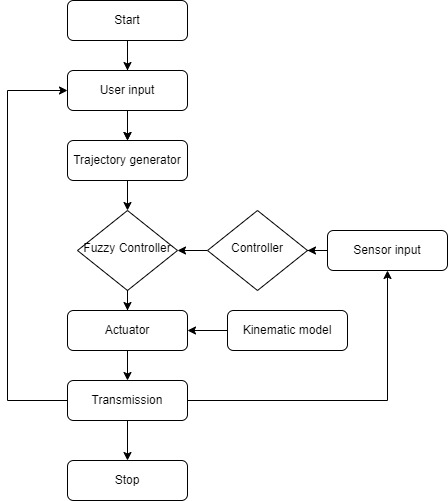
\includegraphics[scale=0.9]{Figures/controller.jpg}
\centering
\caption[Flow chart for Motor Control] {Flow chart for Motor Control}
\label{fig:motorcontrol}
\end{figure}


\begin{figure}[htbp]
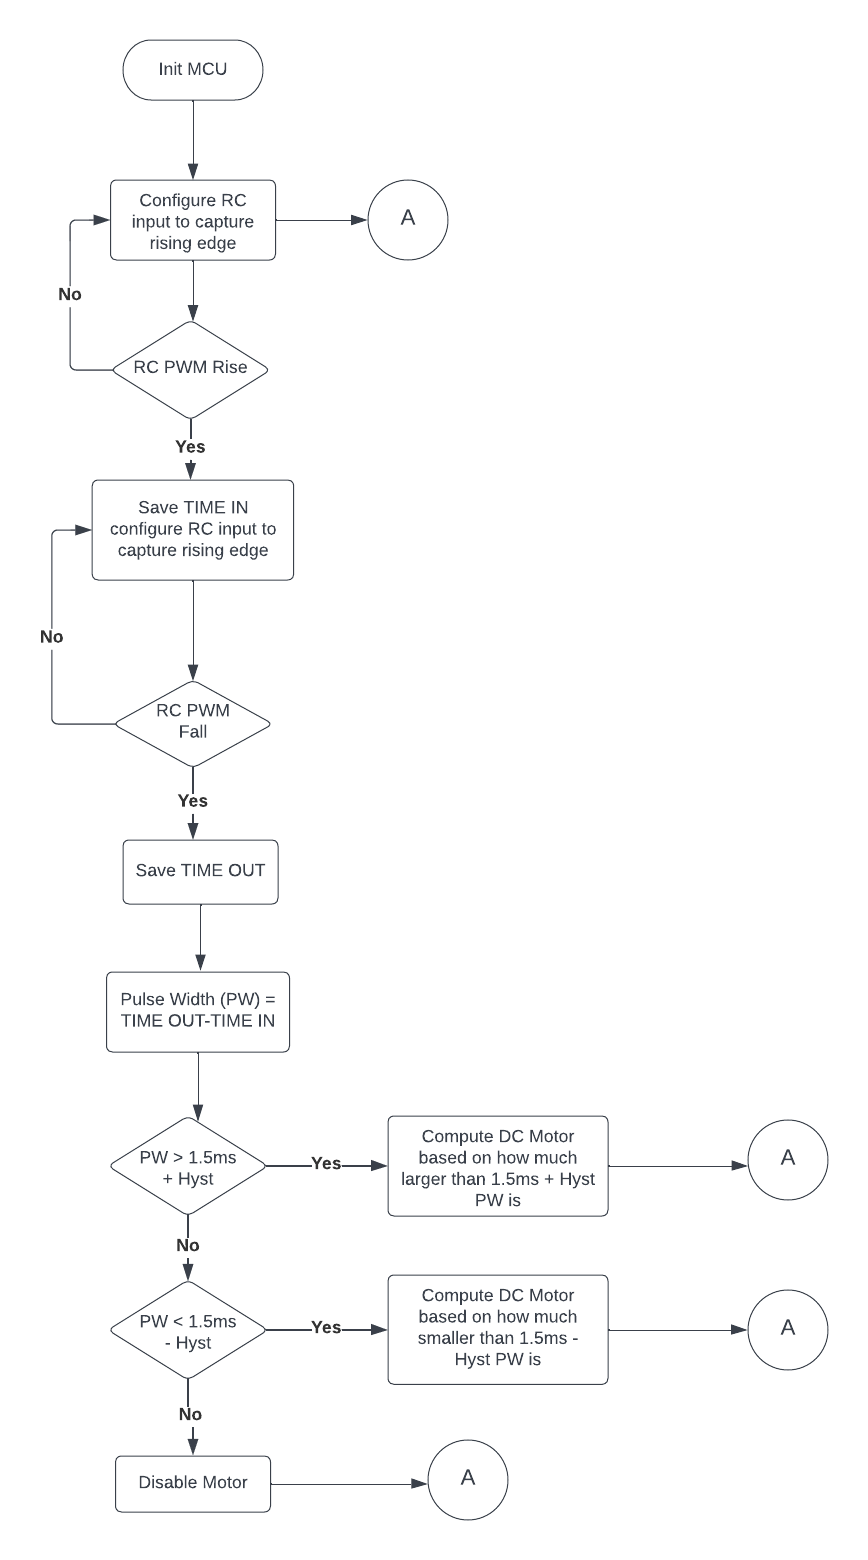
\includegraphics[scale=0.8]{Figures/Blank_diagram.png}
\centering
\caption[Flow chart for Remote Motor Control] {Flow chart for Remote Motor Control}
\label{fig:remotecontrol}
\end{figure}
